\originalchapter{第二次期中考试}
\psource{8.044，2013 春，Exam 2，三题 30/40/30 分。中文题面；据公开官方答案核对的 AI 独立解答。}
\originalsection{1．表面膜熵（30 分）}
\begin{exercise}
水面面积 $A$ 覆盖 $N$ 个有机分子的膜，张力 $\gamma=\gamma_0-N\kb T/(A-bN)+aN^2/A^2$，$C_A=N\kb+N\kb(T/T_0)^2$，参数常数。求 $S(T,A)$ 到一个加性常数，面积功为 $\gamma\dd A$。
\end{exercise}
\begin{solution}
$S_T=C_A/T=N\kb/T+N\kb T/T_0^2$，$S_A=-\gamma_T=N\kb/(A-bN)$，故
\[S=N\kb\ln(T/T_*)+\frac{N\kb T^2}{2T_0^2}+N\kb\ln[(A-bN)/A_*]+S_* .\]
$T_*,A_*$ 使对数无量纲；$a,\gamma_0$ 的温度导数为零，不进入熵。此现象模型不能未经检验外推到零温。
\end{solution}
\originalsection{2．晶场劈裂（40 分）}
\begin{exercise}
$N$ 个相似杂质固定在各晶格位，$L=1$，自由三态简并；晶场使 $m=0$ 能量零、$m=\pm1$ 能量 $\Delta>0$。
(a，10 分) 内能贡献；(b，10 分) 不计算给零温和高温熵；(c，10 分) 热容并画两端行为；(d，10 分) 压缩增大能隙，$\dd\Delta/\dd V=-\gamma\Delta/V$，求杂质对晶格的铺展压。
\end{exercise}
\begin{solution}
$z=1+2e^{-x}$，$x=\Delta/(\kb T)$，固定位置故 $Z=z^N$。
(a) $U=2N\Delta e^{-x}/(1+2e^{-x})$。(b) $S(0)=0$，高温 $S=N\kb\ln3$。(c) $C=2N\kb x^2e^{-x}/(1+2e^{-x})^2$；低温 $2N\kb x^2e^{-x}$，高温 $2N\kb x^2/9$，中间 Schottky 峰。(d) $P=\kb T\partial_V\ln Z=-U\Delta_V/\Delta=\gamma U/V$；符号对应能量随体积降低而增加。
\end{solution}
\begin{center}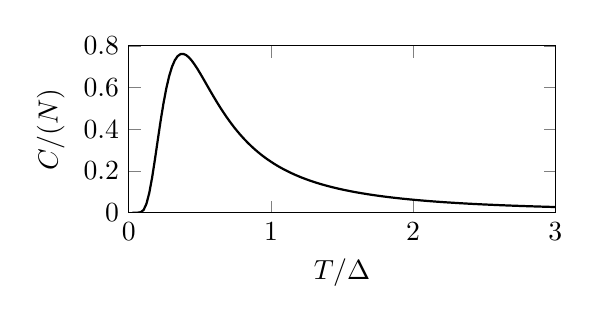
\begin{tikzpicture}\begin{axis}[width=7cm,height=3.7cm,xmin=0,xmax=3,ymin=0,ymax=.8,xlabel={$\kb T/\Delta$},ylabel={$C/(N\kb)$},samples=150]\addplot[domain=.025:3,thick]{2*exp(-1/x)/(x*x*(1+2*exp(-1/x))^2)};\end{axis}\end{tikzpicture}\end{center}
\originalsection{3．内热源与选择吸收球壳（30 分）}
\begin{exercise}
真空中半径 $R$ 球壳由球心半径 $r\ll R$ 的小黑体供热，黑体恒温 $T_H$，球壳向外辐射。
(a，10 分) 壳吸收率 $\alpha=1$、与频率无关时求稳态 $T_S$；随后 $\alpha(\omega)=1$ 当 $0<\omega<\omega_0$，$\omega>\omega_0$ 时完全透明，且 $\hbar\omega_0\ll\kb T_H$。
(b，10 分) 用 Rayleigh--Jeans $u_\omega\simeq\kb T\omega^2/(\pi^2c^3)$ 求吸收总功率；(c，10 分) 再假定 $\hbar\omega_0\ll\kb T_S$ 求稳态壳温。
\end{exercise}
\begin{solution}
(a) 主阶平衡 $4\pi r^2\sigma_{\rm SB}T_H^4=4\pi R^2\sigma_{\rm SB}T_S^4$，$T_S=T_H\sqrt{r/R}$。
(b) Kirchhoff 发射 $e_\omega=cu_\omega/4$，全部从小黑体出的低频功率被壳接收：
\[P_{\rm abs}=4\pi r^2\frac c4\int_0^{\omega_0}\frac{\kb T_H\omega^2}{\pi^2c^3}\dd\omega=\frac{r^2\kb T_H\omega_0^3}{3\pi c^2}.\]
(c) 壳向外的同带功率为同式把 $r^2T_H$ 换为 $R^2T_S$，故 $T_S=T_H(r/R)^2$。须实际检查这更低的温度仍满足 (c) 的 Rayleigh--Jeans 条件，否则应保留 Planck 积分。这里按 $r\ll R$ 忽略壳向小黑体返回的比例 $r^2/R^2$；若计此项，精确平衡分别把 $R^2$ 换成 $R^2+r^2$，主阶结果不变。
\end{solution}
